\appendix
\section{Appendix}
\subsection{Speedup of Speculative Decoding}
As proved in ~\cite{leviathan2023fast}, compared with standard decoding, the expected improvement factor for offline speculative decoding is \(\frac{1-\alpha^{k+1}}{(1-\alpha)(ck+1)}\).
Let the time taken for a single run of \(M_p\) be \(T\). Define \(c\), the cost coefficient, as the ratio of the time taken for a single run of \(M_q\) to that of \(M_p\).
Each execution of lines 7 to 8 takes \(Tck + T\) and, on average, yields \(\frac{1-\alpha^{k+1}}{1-\alpha}\) tokens.
As a result, the average time to produce one token using speculative decoding is given by \(\frac{(ck+1)(1-\alpha)}{1-\alpha^{k+1}}T\). 
In contrast, the time to produce a single token using standard decoding is \(T\). 
Hence, the wallclock time reduction of offline speculative decoding can be described as \(\frac{1-\alpha^{k+1}}{(1-\alpha)(ck+1)}\).

\subsection{Latency Analysis}
\label{appendix:latency-analysis}
Suppose \tool can improve the token acceptance rate from \( \alpha_1 \) to \( \alpha_2 \) %
and $T$ is the generation time for standard decoding. Based on Equation~\ref{eq:gen_len}, this improvement leads to a decrease in the average generation time for each token, transitioning from \( \frac{(ck+1)(1-\alpha_1)}{1-\alpha_{1}^{k+1}}T \) to \( \frac{(ck+1)(1-\alpha_2)}{1-\alpha_{2}^{k+1}}T \). Consequently, this results in a speedup factor of \( \frac{1-\alpha_2^{k+1}}{1-\alpha_1^{k+1}}\frac{1-\alpha_1}{1-\alpha_2} = \frac{1+\alpha_2+\alpha_2^2+...+\alpha_2^{k}}{1+\alpha_1+\alpha_1^2+...+\alpha_1^k}\) compared to standard speculative decoding.

In the aforementioned analysis, we omitted the additional latency due to updating the smaller model for the following reasons:
(1) As illustrated subsequently, the additional computational cost (FLOPs) from the update remains marginal when juxtaposed with the 
computational demands of running the larger model.
(2) Updates are periodic, during times of moderate request loads, the latency for serving individual requests remains largely unaffected. 
Additionally, given that the update operation for the smaller model is considerably less resource-intensive than inference, 
the associated latency might be seamlessly masked, rendering it virtually imperceptible.
Lastly, the processes of updating and inference can even be executed concurrently on separate devices.

\subsection{Flops Analysis}
\label{appendix:flops}
\emph{The FLOPs required to update the draft model are significantly fewer than those needed for inference on a large model.}
Denote \(L\) as the average length of the generated sequence. 
For each verification, the draft model suggests \(k\) tokens. 
The expected length for a single run of the target LLM, denoted as \(a\), can be calculated using Equation~\ref{eq:gen_len}. 
Therefore, \tool undergoes the verification process \(\frac{L}{a}\) times, with each time verifying $k+1$ tokens.
We use \(F_{qfwd}\) to represent the arithmetic operations required by a singular forward run of the draft model for each token, 
and \(F_{pfwd}\) stands for the FLOPs needed for a single forward run of the target model per token.
Therefore, the computational demand (in FLOPs) for the draft and teacher models to handle one request can be expressed as:
$
\text{FLOPs}(draft)  = \frac{L}{a} \times k \times F_{qfwd},
\text{FLOPs}(target) = \frac{L}{a} \times (k+1) \times F_{pfwd}.
$
Let's consider the FLOPs required to update the student model per token as \(F_{qbwd}\). The cumulative FLOPs necessary to process \(I\) requests is given by:
\[
\frac{LI}{a} \times \left[k \times F_{qfwd} + (k+1) \times F_{pfwd}\right] + I \times L \times F_{qbwd}.
\]
Based on the findings of \cite{kaplan2020scaling}, training is approximately three times costlier than inference. This translates to roughly 6 FLOPs per parameter for training on a single token and 2 FLOPs per parameter for inferring on one token. Thus, we can simplify the total FLOPs expression to:
\begin{equation}
    \frac{LI}{a}\left[(k + 3a) \times F_{qfwd} + (k+1) \times F_{pfwd}\right].
\end{equation}

The proportion of FLOPs needed to run the target model to that of the draft model is given by:
\[
\frac{(k+1)\times F_{pfwd}}{(k+3a)\times F_{qfwd}}.
\]
For the two model pairs evaluated, assuming an average of 5 proposed tokens per run: 
(1) (LLaMA-160M, Vicuna7B) with an average acceptance rate of 0.71, the ratio is approximately \( \frac{(5+1) \times 7B}{(5+3 \times 3) \times 160M} = 18.75 \).
(2) (T5-small 80M, Flan-T5-XL 3B), with an average acceptance rate of 0.76, the ratio is roughly \( \frac{(5+1) \times 3B}{(5+3 \times 4.3) \times 80M} = 12.6 \).

\emph{In practical systems, the FLOPs required for inference are significantly below the machine's capacity.} 
Consider the LMSYS-Chat-1M~\cite{zheng2023lmsyschat1m}. It comprises traces spanning 125 days with 1000,000 requests, averaging less than 2,000 tokens per request (including both prompts and responses).
When serving a 30B model with 8 A100 GPUs, the FLOPs consumed per second can be estimated as (Still, we estimate 2 FLOPs per token per parameter):
\[ \frac{2000 \times 1000,000}{125 \times 24 \times 3600} \times 30 \times 10^9 \times 2 = 5.5 \times 10^9 \text{ FLOPs or 5.5 GFLOPs} \]
On the other hand, 8 A100 GPUs offer a combined capacity of \( 8 \times 312 \text{ TFLOPs} \), and the computational utilization is notably low. 
While Arena (the platform that generates LMSYS-Chat-1M) may not be the most efficient and might lack substantial traffic, it's the only publicly accessible LLM service trace. 
Even after amplifying the load multiple times, based on the above calculations, the computation efficiency remains limited.


\subsection{Data Mix}
\label{appendix:data-mix}
Moreover, there is a question of whether the draft model, once adapted to the new distribution, might lose its prior knowledge. 
To probe this, we conducted an experiment mixing 2k prompts each from the Gsm8k and Alpaca-finance datasets. 
During online serving, for the initial 2k requests, we only update the model based on data from the Gsm8k dataset. 
For the subsequent half of the requests, we restrict updates solely to data from the Alpaca-finance dataset. 
We then provide the average token acceptance rates for all requests, segmented by their data source (Gsm8k versus Alpaca-finance).
As depicted in Figure~\ref{fig:mix}, the token acceptance rate for Gsm8k increases as the draft model 
is exposed to more data. Conversely, the acceptance rate (\(\alpha\)) for the Alpaca-finance dataset remains consistent. 
This is anticipated since we only update the draft model using Gsm8k data. In the latter half of the dataset, 
the token acceptance rate for the Alpaca-finance dataset also shows an uptrend. Intriguingly, the rate for Gsm8k remains consistent, 
suggesting that the draft model retains its learned knowledge without showing signs of forgetting.

\begin{figure}      
    \centering
    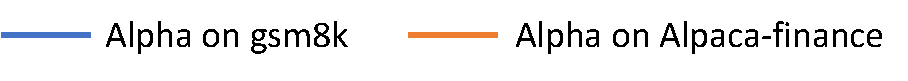
\includegraphics[width=0.48\linewidth]{figures/appendix_legend.pdf} \\
    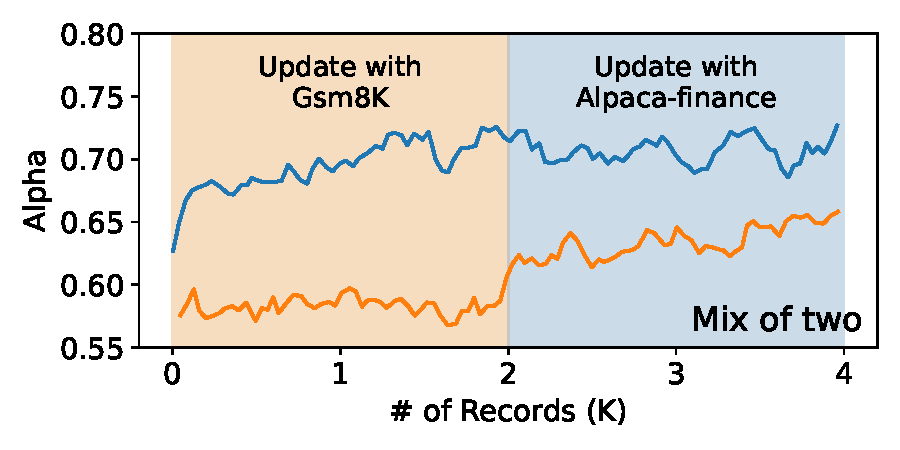
\includegraphics[width=0.48\linewidth]{figures/mix.pdf}
    \caption{Mix of distributions.}
    \label{fig:mix}
\end{figure}

\subsection{Data Preparation for Distribution Shift Analysi}
To emulate this shift in distribution, 
\label{appendix:distribution-shift}
we select 2k prompts from each dataset under evaluation. T
he data from the four datasets are amalgamated by direct concatenation, 
such that the records from $i\times2k$ to $(i+1)\times2k$ belong solely to dataset 
$i$. 

\subsection{Arena Dataset}
\label{appendix:arena}
For expedited experimental evaluation, we randomly sample a subset with 10K records
from LMSYS-Chat-1M~\cite{zheng2023lmsyschat1m}, 
a comprehensive real-world LLM conversation dataset. This dataset encompasses interactions with 25 models spanning 
from April to August 2023 and features conversations in over 150 languages. For all experiments, we only pick conversations for Vicuna models.

